% Build: pdflatex main; bibtex main; pdflatex main; pdflatex main.

\documentclass[sigconf,nonacm]{acmart}

\usepackage{listings}
\usepackage{xcolor}
\usepackage{booktabs}
\usepackage{amsmath}
% acmart's font setup already defines \Bbbk; relax it before amssymb
% reloads it to avoid "Command \Bbbk already defined".
\let\Bbbk\relax
\usepackage{amssymb}
\usepackage{algorithm}
\usepackage{algpseudocode}
\usepackage{tikz}
\usetikzlibrary{arrows.meta, positioning, shapes.geometric}

% Suppress ACM conference matter for a class capstone.  Drop the
% \settopmatter and the [nonacm] class option if submitting through
% an actual ACM venue; see BUILD_NOTES.md.
\settopmatter{printacmref=false, printccs=false, printfolios=true}
\setcopyright{none}
\renewcommand\footnotetextcopyrightpermission[1]{}
\pagestyle{plain}

\definecolor{lstbg}{HTML}{F7F7F7}
\definecolor{lstkw}{HTML}{0033B3}
\definecolor{lstcm}{HTML}{6A737D}
\definecolor{lststr}{HTML}{067D17}

\lstdefinestyle{shellstyle}{
  language=bash,
  basicstyle=\ttfamily\small,
  keywordstyle=\color{lstkw}\bfseries,
  commentstyle=\color{lstcm}\itshape,
  stringstyle=\color{lststr},
  backgroundcolor=\color{lstbg},
  breaklines=true,
  columns=fullflexible,
  keepspaces=true,
  showstringspaces=false,
  frame=single,
  rulecolor=\color{black!20},
  xleftmargin=0.5em,
  xrightmargin=0.5em,
  aboveskip=0.6em,
  belowskip=0.6em,
}

\lstdefinestyle{pystyle}{
  language=Python,
  basicstyle=\ttfamily\small,
  keywordstyle=\color{lstkw}\bfseries,
  commentstyle=\color{lstcm}\itshape,
  stringstyle=\color{lststr},
  backgroundcolor=\color{lstbg},
  breaklines=true,
  columns=fullflexible,
  keepspaces=true,
  showstringspaces=false,
  frame=single,
  rulecolor=\color{black!20},
  xleftmargin=0.5em,
  xrightmargin=0.5em,
  aboveskip=0.6em,
  belowskip=0.6em,
}

\lstdefinestyle{tsvstyle}{
  basicstyle=\ttfamily\footnotesize,
  backgroundcolor=\color{lstbg},
  breaklines=false,
  columns=fullflexible,
  keepspaces=true,
  frame=single,
  rulecolor=\color{black!20},
  xleftmargin=0.5em,
  xrightmargin=0.5em,
}

\title{Extending the Dynamic Regulatory Events Miner to Methylation
       Dynamics: A Transcription-Factor-to-DMR Prior Framework for
       Brain Cell Lineages}

\author{Jon Paino}
\affiliation{%
  \institution{University of California, Los Angeles}
  \city{Los Angeles}
  \state{California}
  \country{USA}}
\email{jonpaino@cs.ucla.edu}

\begin{document}

\begin{abstract}
The Dynamic Regulatory Events Miner (DREM) is an Input-Output Hidden
Markov Model originally formulated over time-series gene expression,
in which a per-time-point dynamic measurement is paired with a static
TF-to-gene prior. This report describes a methodological extension of
the DREM framework to a different dynamic substrate: DNA methylation
$\beta$-values measured along the developmental trajectories of human
brain cell lineages. Because DREM was designed assuming expression as
the dynamic input, this work also evaluates whether DREM remains
functional when methylation, rather than expression, is supplied as
the temporal substrate. The substrate change forces a corresponding
change in the prior: the TF-to-gene table is replaced by a TF-to-DMR
table built by intersecting ChIP-Atlas peak BEDs with
lineage-specific DMR BEDs, retaining DMR identity rather than
collapsing to gene-level annotations. This report describes the
TF--DMR prior framework, the curated accession whitelist (172 records,
spanning SRX, ERX, and DRX entries) that defines the transcription
factor coverage, a BrainSpan RPKM expression filter that restricts the
prior to TFs operative in developing human brain, and a parameterized
regeneration pipeline that produces five lineage-specific TF--DMR
priors used in a BICAN methylation analysis. Applied to neural
differentiation trajectories in the BICAN human brain methylation
atlas, the resulting DREM models recovered polycomb-antagonizing
SWI/SNF chromatin-remodeler subunits (SMARCA4, SMARCB1) and early
patterning TFs (ASCL1,
SOX2) at regions gaining mCG in mid-gestation, identified SOX10 and
MEF2C as lineage-specific drivers of methylation change in the
OPC-to-ODC and MGE-derived inhibitory neuron arcs respectively, and
reiterated activity-dependent AP-1 enrichment (FOSL2, FOS, JUNB) at
regions distinguishing striosomal from matrix MSN differentiation
programs in DRD1-BACH2 versus DRD1-EPHA4 trajectories.

\end{abstract}

\maketitle

\section{Introduction}
\label{sec:intro}

Dynamic regulatory networks underlie the transitions that distinguish
one neural cell type from another during human brain development. A
standard inferential question is which transcription factors (TFs)
drive the bifurcations along a lineage trajectory, given a dynamic
measurement of cell state and a candidate set of TF binding events.
DREM~\cite{ernst2007dremoriginal,schulz2012drem2} addresses this
question for time-series gene expression: an Input-Output Hidden
Markov Model fits the temporal expression of each gene, and a
logistic regression at each split node uses TF--gene binding evidence
to annotate the bifurcation. The framework is agnostic about which
biological measurement enters the dynamic input layer, but the
default workflow assumes the dynamic substrate is gene expression and
the prior connects TFs to genes through promoter windows.

The BICAN (Brain Initiative Cell Atlas Network) multi-modal
atlas of the developing human brain~\cite{bican2026manuscript}
produces a different dynamic
substrate: DNA methylation $\beta$-values measured at differentially
methylated regions (DMRs) along each cell-type lineage. Methylation
changes are localized to the DMRs themselves, not to the
$\pm 2$~kb windows around transcription start sites that the
default TF--gene prior is built from. Applying DREM to methylation
dynamics therefore raises two questions. The first is methodological:
how to construct a prior whose substrate matches the substrate of the
dynamic measurement rather than the gene-promoter substrate DREM
assumes by default. The second is whether DREM's IOHMM, which was
designed and validated on gene expression, remains functional at all
when methylation $\beta$ rather than expression is supplied as the
dynamic input. This report addresses both.
% =====================================================================
% BACKGROUND SECTION
% Drop in via % =====================================================================
% BACKGROUND SECTION
% Drop in via % =====================================================================
% BACKGROUND SECTION
% Drop in via \input{background_section} from main.tex.
% Assumes acmart sigconf and the bib entries provided in references.bib.
% =====================================================================

\section{Background}
\label{sec:background}

\subsection{DREM and the IOHMM framework}

The Dynamic Regulatory Events Miner (DREM) was introduced by Ernst et al.~\cite{ernst2007dremoriginal} as a method for reconstructing dynamic gene regulatory networks (GRNs) from time-series expression data. The model is an Input-Output Hidden Markov Model (IOHMM) over the temporal expression profile of each gene. Hidden states correspond to nodes in the dynamic network; observations are the per-time-point expression values of a gene; and the transition probabilities at each node are produced by a logistic regression classifier whose inputs are protein-DNA interaction values (the static input layer). When a node has more than one outgoing transition, that node is a \emph{split node}: a point along the trajectory (in real sampling time, or in pseudotime when DREM is run on a pseudotime-ordered series) at which a co-expressed group of genes diverges into multiple paths. The TF annotations at each split are based on the assignment of genes to their most likely path, which is determined by inference over the entire model. The logistic regression at each split then identifies which transcription factors (TFs) most distinguish genes assigned to one outgoing path from genes assigned to the other~\cite{ernst2007dremoriginal, schulz2012drem2}.

DREM 2.0~\cite{schulz2012drem2} extended the original framework with packaged protein-DNA interaction data for several species, support for continuous binding values, an option to scale TF effects by their own expression at each time point, dynamic (time-point-specific) input layers, and integrated motif discovery. The interactive GUI for inspection of the learned model was present in the original DREM and received smaller modifications in 2.0. The two pieces of input that the user supplies for a typical run are (i) a time-series matrix of dynamic measurements indexed by gene and time point, and (ii) a static or dynamic prior file in three columns: \texttt{TF}, \texttt{Gene}, \texttt{Input}, where the \texttt{Input} column is the binding value used by the logistic regression classifier (binary or continuous).

The first input encodes \emph{what is changing} along the trajectory. The second input encodes \emph{which regulators are candidates to explain the change}. DREM was originally designed assuming the first input is gene expression; whether it remains functional when methylation is supplied as the dynamic substrate instead is one of the questions this work evaluates. In principle the framework is agnostic about what biological measurement appears in the first input as long as it varies along time or pseudotime, and about what the prior connects as long as the rows of the dynamic matrix line up with the entities the prior maps to. Although DREM 2.0 supports dynamic (time-point-specific) priors, the work here uses a single static prior throughout. This separation between the dynamic substrate and the static prior, together with a correspondence between the row identifiers of the dynamic matrix and the entities indexed in the prior, is what the modality extension exploits.

\subsection{Methylation dynamics in the BICAN brain atlas}

The BICAN U01 project assembled a multi-modal single-cell atlas of the developing human brain spanning mid-gestation through 7 months postnatal, profiling DNA methylation (mCG) and three-dimensional chromatin contacts (3C) jointly via snm3C-seq~\cite{bican2026manuscript}. The developmental BICAN data were integrated with previously collected adult brain data, so that each lineage spans from a fetal progenitor state through to the corresponding adult cell type. Within that atlas, lineage trajectories were constructed for major neural cell types, including medial ganglionic eminence (MGE)-derived parvalbumin (PV) interneurons (MGE\_PVALB), two medium spiny neuron (MSN) subtypes (MSN\_DRD1\_BACH2 and MSN\_DRD1\_EPHA4), the oligodendrocyte precursor cell (OPC) to oligodendrocyte (ODC) differentiation arc (OPC\_ODC), and an immature caudal ganglionic eminence-derived LAMP5 inhibitory neuron lineage (eCGE\_LAMP5, where CGE denotes the caudal ganglionic eminence and the \texttt{e} prefix denotes the immature stage).

Differentially methylated regions (DMRs) were called by methylpy pairwise between adjacent developmental stages along each lineage (3T $\rightarrow$ 1m $\rightarrow$ 4--7m $\rightarrow$ adult). For each pairwise comparison, methylpy reports the differential regions from the perspective of each side, labeling both directions as ``hypo'' relative to the higher-methylation side. The merged lineage BED used here (despite its \texttt{\_hypo\_merged} filename) is the union of both directions of those pairwise comparisons, so it captures regulatory elements that lose mCG and regulatory elements that gain mCG along the trajectory, rather than demethylation events alone.

The dynamic measurement of interest in this setting is methylation $\beta$ at each DMR, indexed by developmental-stage cluster ordered along the lineage trajectory. This is the natural input to a DREM-style IOHMM if one wants to ask which TFs drive the methylation transitions at lineage bifurcations. The challenge is that DREM's standard prior is a TF-to-gene table built by intersecting ChIP-seq peaks with promoter windows, which is appropriate when the dynamic substrate is gene expression but mismatched when the dynamic substrate is methylation: the regions where methylation is changing are the DMRs themselves, not the $\pm 2$ kb windows around transcription start sites. Resolving this mismatch is the substantive methodological problem the rest of this report addresses.

\subsection{ChIP-Atlas and the TF binding evidence base}

The TF binding evidence used to build the prior comes from ChIP-Atlas~\cite{oki2018chipatlas}, a public reanalysis pipeline that uniformly processes ChIP-seq, ATAC-seq, and DNase-seq experiments deposited in NCBI SRA and similar archives. For each experiment, ChIP-Atlas publishes a peak BED file at multiple stringency thresholds and an experiment metadata table linking each experiment accession (SRX, ERX, or DRX, depending on the archive in which the experiment was originally deposited) to a target antigen and cell type. The peak BEDs are the substrate from which the TF-DMR prior is constructed: the framework intersects per-experiment peaks with lineage-specific DMR BEDs to produce a (TF, DMR) graph weighted by which transcription factors show binding evidence in the genomic regions where methylation is dynamic along each lineage. ChIP-Atlas's metadata also requires curation, since the ``antigen'' column includes entries that are not sequence-specific transcription factors (epitope tags, oxidative modifications, GFP fusions, histone modifications); these typically reflect a different experimental approach in which the intended target is annotated in a different metadata column, rather than annotation errors. The accession set used here filters these out; the antigens that remain are predominantly sequence-specific transcription factors, together with a minority of non-sequence-specific chromatin-associated proteins (for example cohesin and Mediator subunits and SWI/SNF remodeler subunits) that the curation procedure retained on the strength of their ChIP-seq evidence. Section~\ref{sec:framework:tfset} enumerates this composition.

\subsection{BrainSpan as a brain-relevance filter}

ChIP-Atlas aggregates experiments across all available cell types and tissues, so a TF that has many peaks in the genome may nonetheless be biologically irrelevant in the brain. To restrict the prior to TFs that are operative in human neural tissue, this work uses the BrainSpan developmental transcriptome~\cite{miller2014brainspan} as a second filter. BrainSpan provides bulk RNA-seq from 524 samples spanning multiple brain regions and developmental stages from 8 post-conceptional weeks through adulthood, processed to a per-gene RPKM matrix. A TF passes the filter if its mean RPKM across the BrainSpan samples exceeds a threshold. The threshold is chosen so that borderline regulators of demonstrated brain importance are retained: REST, for example, has a BrainSpan mean RPKM of $1.29$, and the threshold used here is set just below such biologically anchored points so that REST and similar regulators are not excluded. The choice is discussed in Section~\ref{sec:framework}.

\subsection{Related approaches}

Several approaches use temporal expression data to reconstruct regulatory networks. Friedman's dynamic Bayesian networks~\cite{friedman1998dbn} provide a formally clean framework for learning network structure from time-series expression but do not natively incorporate a static TF-DNA prior, and the structure-learning scales poorly to the hundreds of TFs that typical regulatory analyses require. Network Component Analysis~\cite{liao2003nca} does combine static interaction data, in the form of a TF-promoter connectivity matrix derived from ChIP-chip or literature, with expression measurements, but its matrix-factorization decomposition treats the time index as exchangeable rather than ordered. DREM's IOHMM occupies a useful middle ground: it respects time ordering, scales to hundreds of TFs through the logistic regression at split nodes, and produces an interpretable graphical model with TF annotations attached to specific bifurcation events. The work presented here treats DREM's IOHMM as a fixed inferential engine and focuses entirely on the prior side of the input pair, swapping the gene-substrate prior for a DMR-substrate prior matched to the methylation dynamic measurement.

% =====================================================================
% End of background section
% =====================================================================
 from main.tex.
% Assumes acmart sigconf and the bib entries provided in references.bib.
% =====================================================================

\section{Background}
\label{sec:background}

\subsection{DREM and the IOHMM framework}

The Dynamic Regulatory Events Miner (DREM) was introduced by Ernst et al.~\cite{ernst2007dremoriginal} as a method for reconstructing dynamic gene regulatory networks (GRNs) from time-series expression data. The model is an Input-Output Hidden Markov Model (IOHMM) over the temporal expression profile of each gene. Hidden states correspond to nodes in the dynamic network; observations are the per-time-point expression values of a gene; and the transition probabilities at each node are produced by a logistic regression classifier whose inputs are protein-DNA interaction values (the static input layer). When a node has more than one outgoing transition, that node is a \emph{split node}: a point along the trajectory (in real sampling time, or in pseudotime when DREM is run on a pseudotime-ordered series) at which a co-expressed group of genes diverges into multiple paths. The TF annotations at each split are based on the assignment of genes to their most likely path, which is determined by inference over the entire model. The logistic regression at each split then identifies which transcription factors (TFs) most distinguish genes assigned to one outgoing path from genes assigned to the other~\cite{ernst2007dremoriginal, schulz2012drem2}.

DREM 2.0~\cite{schulz2012drem2} extended the original framework with packaged protein-DNA interaction data for several species, support for continuous binding values, an option to scale TF effects by their own expression at each time point, dynamic (time-point-specific) input layers, and integrated motif discovery. The interactive GUI for inspection of the learned model was present in the original DREM and received smaller modifications in 2.0. The two pieces of input that the user supplies for a typical run are (i) a time-series matrix of dynamic measurements indexed by gene and time point, and (ii) a static or dynamic prior file in three columns: \texttt{TF}, \texttt{Gene}, \texttt{Input}, where the \texttt{Input} column is the binding value used by the logistic regression classifier (binary or continuous).

The first input encodes \emph{what is changing} along the trajectory. The second input encodes \emph{which regulators are candidates to explain the change}. DREM was originally designed assuming the first input is gene expression; whether it remains functional when methylation is supplied as the dynamic substrate instead is one of the questions this work evaluates. In principle the framework is agnostic about what biological measurement appears in the first input as long as it varies along time or pseudotime, and about what the prior connects as long as the rows of the dynamic matrix line up with the entities the prior maps to. Although DREM 2.0 supports dynamic (time-point-specific) priors, the work here uses a single static prior throughout. This separation between the dynamic substrate and the static prior, together with a correspondence between the row identifiers of the dynamic matrix and the entities indexed in the prior, is what the modality extension exploits.

\subsection{Methylation dynamics in the BICAN brain atlas}

The BICAN U01 project assembled a multi-modal single-cell atlas of the developing human brain spanning mid-gestation through 7 months postnatal, profiling DNA methylation (mCG) and three-dimensional chromatin contacts (3C) jointly via snm3C-seq~\cite{bican2026manuscript}. The developmental BICAN data were integrated with previously collected adult brain data, so that each lineage spans from a fetal progenitor state through to the corresponding adult cell type. Within that atlas, lineage trajectories were constructed for major neural cell types, including medial ganglionic eminence (MGE)-derived parvalbumin (PV) interneurons (MGE\_PVALB), two medium spiny neuron (MSN) subtypes (MSN\_DRD1\_BACH2 and MSN\_DRD1\_EPHA4), the oligodendrocyte precursor cell (OPC) to oligodendrocyte (ODC) differentiation arc (OPC\_ODC), and an immature caudal ganglionic eminence-derived LAMP5 inhibitory neuron lineage (eCGE\_LAMP5, where CGE denotes the caudal ganglionic eminence and the \texttt{e} prefix denotes the immature stage).

Differentially methylated regions (DMRs) were called by methylpy pairwise between adjacent developmental stages along each lineage (3T $\rightarrow$ 1m $\rightarrow$ 4--7m $\rightarrow$ adult). For each pairwise comparison, methylpy reports the differential regions from the perspective of each side, labeling both directions as ``hypo'' relative to the higher-methylation side. The merged lineage BED used here (despite its \texttt{\_hypo\_merged} filename) is the union of both directions of those pairwise comparisons, so it captures regulatory elements that lose mCG and regulatory elements that gain mCG along the trajectory, rather than demethylation events alone.

The dynamic measurement of interest in this setting is methylation $\beta$ at each DMR, indexed by developmental-stage cluster ordered along the lineage trajectory. This is the natural input to a DREM-style IOHMM if one wants to ask which TFs drive the methylation transitions at lineage bifurcations. The challenge is that DREM's standard prior is a TF-to-gene table built by intersecting ChIP-seq peaks with promoter windows, which is appropriate when the dynamic substrate is gene expression but mismatched when the dynamic substrate is methylation: the regions where methylation is changing are the DMRs themselves, not the $\pm 2$ kb windows around transcription start sites. Resolving this mismatch is the substantive methodological problem the rest of this report addresses.

\subsection{ChIP-Atlas and the TF binding evidence base}

The TF binding evidence used to build the prior comes from ChIP-Atlas~\cite{oki2018chipatlas}, a public reanalysis pipeline that uniformly processes ChIP-seq, ATAC-seq, and DNase-seq experiments deposited in NCBI SRA and similar archives. For each experiment, ChIP-Atlas publishes a peak BED file at multiple stringency thresholds and an experiment metadata table linking each experiment accession (SRX, ERX, or DRX, depending on the archive in which the experiment was originally deposited) to a target antigen and cell type. The peak BEDs are the substrate from which the TF-DMR prior is constructed: the framework intersects per-experiment peaks with lineage-specific DMR BEDs to produce a (TF, DMR) graph weighted by which transcription factors show binding evidence in the genomic regions where methylation is dynamic along each lineage. ChIP-Atlas's metadata also requires curation, since the ``antigen'' column includes entries that are not sequence-specific transcription factors (epitope tags, oxidative modifications, GFP fusions, histone modifications); these typically reflect a different experimental approach in which the intended target is annotated in a different metadata column, rather than annotation errors. The accession set used here filters these out; the antigens that remain are predominantly sequence-specific transcription factors, together with a minority of non-sequence-specific chromatin-associated proteins (for example cohesin and Mediator subunits and SWI/SNF remodeler subunits) that the curation procedure retained on the strength of their ChIP-seq evidence. Section~\ref{sec:framework:tfset} enumerates this composition.

\subsection{BrainSpan as a brain-relevance filter}

ChIP-Atlas aggregates experiments across all available cell types and tissues, so a TF that has many peaks in the genome may nonetheless be biologically irrelevant in the brain. To restrict the prior to TFs that are operative in human neural tissue, this work uses the BrainSpan developmental transcriptome~\cite{miller2014brainspan} as a second filter. BrainSpan provides bulk RNA-seq from 524 samples spanning multiple brain regions and developmental stages from 8 post-conceptional weeks through adulthood, processed to a per-gene RPKM matrix. A TF passes the filter if its mean RPKM across the BrainSpan samples exceeds a threshold. The threshold is chosen so that borderline regulators of demonstrated brain importance are retained: REST, for example, has a BrainSpan mean RPKM of $1.29$, and the threshold used here is set just below such biologically anchored points so that REST and similar regulators are not excluded. The choice is discussed in Section~\ref{sec:framework}.

\subsection{Related approaches}

Several approaches use temporal expression data to reconstruct regulatory networks. Friedman's dynamic Bayesian networks~\cite{friedman1998dbn} provide a formally clean framework for learning network structure from time-series expression but do not natively incorporate a static TF-DNA prior, and the structure-learning scales poorly to the hundreds of TFs that typical regulatory analyses require. Network Component Analysis~\cite{liao2003nca} does combine static interaction data, in the form of a TF-promoter connectivity matrix derived from ChIP-chip or literature, with expression measurements, but its matrix-factorization decomposition treats the time index as exchangeable rather than ordered. DREM's IOHMM occupies a useful middle ground: it respects time ordering, scales to hundreds of TFs through the logistic regression at split nodes, and produces an interpretable graphical model with TF annotations attached to specific bifurcation events. The work presented here treats DREM's IOHMM as a fixed inferential engine and focuses entirely on the prior side of the input pair, swapping the gene-substrate prior for a DMR-substrate prior matched to the methylation dynamic measurement.

% =====================================================================
% End of background section
% =====================================================================
 from main.tex.
% Assumes acmart sigconf and the bib entries provided in references.bib.
% =====================================================================

\section{Background}
\label{sec:background}

\subsection{DREM and the IOHMM framework}

The Dynamic Regulatory Events Miner (DREM) was introduced by Ernst et al.~\cite{ernst2007dremoriginal} as a method for reconstructing dynamic gene regulatory networks (GRNs) from time-series expression data. The model is an Input-Output Hidden Markov Model (IOHMM) over the temporal expression profile of each gene. Hidden states correspond to nodes in the dynamic network; observations are the per-time-point expression values of a gene; and the transition probabilities at each node are produced by a logistic regression classifier whose inputs are protein-DNA interaction values (the static input layer). When a node has more than one outgoing transition, that node is a \emph{split node}: a point along the trajectory (in real sampling time, or in pseudotime when DREM is run on a pseudotime-ordered series) at which a co-expressed group of genes diverges into multiple paths. The TF annotations at each split are based on the assignment of genes to their most likely path, which is determined by inference over the entire model. The logistic regression at each split then identifies which transcription factors (TFs) most distinguish genes assigned to one outgoing path from genes assigned to the other~\cite{ernst2007dremoriginal, schulz2012drem2}.

DREM 2.0~\cite{schulz2012drem2} extended the original framework with packaged protein-DNA interaction data for several species, support for continuous binding values, an option to scale TF effects by their own expression at each time point, dynamic (time-point-specific) input layers, and integrated motif discovery. The interactive GUI for inspection of the learned model was present in the original DREM and received smaller modifications in 2.0. The two pieces of input that the user supplies for a typical run are (i) a time-series matrix of dynamic measurements indexed by gene and time point, and (ii) a static or dynamic prior file in three columns: \texttt{TF}, \texttt{Gene}, \texttt{Input}, where the \texttt{Input} column is the binding value used by the logistic regression classifier (binary or continuous).

The first input encodes \emph{what is changing} along the trajectory. The second input encodes \emph{which regulators are candidates to explain the change}. DREM was originally designed assuming the first input is gene expression; whether it remains functional when methylation is supplied as the dynamic substrate instead is one of the questions this work evaluates. In principle the framework is agnostic about what biological measurement appears in the first input as long as it varies along time or pseudotime, and about what the prior connects as long as the rows of the dynamic matrix line up with the entities the prior maps to. Although DREM 2.0 supports dynamic (time-point-specific) priors, the work here uses a single static prior throughout. This separation between the dynamic substrate and the static prior, together with a correspondence between the row identifiers of the dynamic matrix and the entities indexed in the prior, is what the modality extension exploits.

\subsection{Methylation dynamics in the BICAN brain atlas}

The BICAN U01 project assembled a multi-modal single-cell atlas of the developing human brain spanning mid-gestation through 7 months postnatal, profiling DNA methylation (mCG) and three-dimensional chromatin contacts (3C) jointly via snm3C-seq~\cite{bican2026manuscript}. The developmental BICAN data were integrated with previously collected adult brain data, so that each lineage spans from a fetal progenitor state through to the corresponding adult cell type. Within that atlas, lineage trajectories were constructed for major neural cell types, including medial ganglionic eminence (MGE)-derived parvalbumin (PV) interneurons (MGE\_PVALB), two medium spiny neuron (MSN) subtypes (MSN\_DRD1\_BACH2 and MSN\_DRD1\_EPHA4), the oligodendrocyte precursor cell (OPC) to oligodendrocyte (ODC) differentiation arc (OPC\_ODC), and an immature caudal ganglionic eminence-derived LAMP5 inhibitory neuron lineage (eCGE\_LAMP5, where CGE denotes the caudal ganglionic eminence and the \texttt{e} prefix denotes the immature stage).

Differentially methylated regions (DMRs) were called by methylpy pairwise between adjacent developmental stages along each lineage (3T $\rightarrow$ 1m $\rightarrow$ 4--7m $\rightarrow$ adult). For each pairwise comparison, methylpy reports the differential regions from the perspective of each side, labeling both directions as ``hypo'' relative to the higher-methylation side. The merged lineage BED used here (despite its \texttt{\_hypo\_merged} filename) is the union of both directions of those pairwise comparisons, so it captures regulatory elements that lose mCG and regulatory elements that gain mCG along the trajectory, rather than demethylation events alone.

The dynamic measurement of interest in this setting is methylation $\beta$ at each DMR, indexed by developmental-stage cluster ordered along the lineage trajectory. This is the natural input to a DREM-style IOHMM if one wants to ask which TFs drive the methylation transitions at lineage bifurcations. The challenge is that DREM's standard prior is a TF-to-gene table built by intersecting ChIP-seq peaks with promoter windows, which is appropriate when the dynamic substrate is gene expression but mismatched when the dynamic substrate is methylation: the regions where methylation is changing are the DMRs themselves, not the $\pm 2$ kb windows around transcription start sites. Resolving this mismatch is the substantive methodological problem the rest of this report addresses.

\subsection{ChIP-Atlas and the TF binding evidence base}

The TF binding evidence used to build the prior comes from ChIP-Atlas~\cite{oki2018chipatlas}, a public reanalysis pipeline that uniformly processes ChIP-seq, ATAC-seq, and DNase-seq experiments deposited in NCBI SRA and similar archives. For each experiment, ChIP-Atlas publishes a peak BED file at multiple stringency thresholds and an experiment metadata table linking each experiment accession (SRX, ERX, or DRX, depending on the archive in which the experiment was originally deposited) to a target antigen and cell type. The peak BEDs are the substrate from which the TF-DMR prior is constructed: the framework intersects per-experiment peaks with lineage-specific DMR BEDs to produce a (TF, DMR) graph weighted by which transcription factors show binding evidence in the genomic regions where methylation is dynamic along each lineage. ChIP-Atlas's metadata also requires curation, since the ``antigen'' column includes entries that are not sequence-specific transcription factors (epitope tags, oxidative modifications, GFP fusions, histone modifications); these typically reflect a different experimental approach in which the intended target is annotated in a different metadata column, rather than annotation errors. The accession set used here filters these out; the antigens that remain are predominantly sequence-specific transcription factors, together with a minority of non-sequence-specific chromatin-associated proteins (for example cohesin and Mediator subunits and SWI/SNF remodeler subunits) that the curation procedure retained on the strength of their ChIP-seq evidence. Section~\ref{sec:framework:tfset} enumerates this composition.

\subsection{BrainSpan as a brain-relevance filter}

ChIP-Atlas aggregates experiments across all available cell types and tissues, so a TF that has many peaks in the genome may nonetheless be biologically irrelevant in the brain. To restrict the prior to TFs that are operative in human neural tissue, this work uses the BrainSpan developmental transcriptome~\cite{miller2014brainspan} as a second filter. BrainSpan provides bulk RNA-seq from 524 samples spanning multiple brain regions and developmental stages from 8 post-conceptional weeks through adulthood, processed to a per-gene RPKM matrix. A TF passes the filter if its mean RPKM across the BrainSpan samples exceeds a threshold. The threshold is chosen so that borderline regulators of demonstrated brain importance are retained: REST, for example, has a BrainSpan mean RPKM of $1.29$, and the threshold used here is set just below such biologically anchored points so that REST and similar regulators are not excluded. The choice is discussed in Section~\ref{sec:framework}.

\subsection{Related approaches}

Several approaches use temporal expression data to reconstruct regulatory networks. Friedman's dynamic Bayesian networks~\cite{friedman1998dbn} provide a formally clean framework for learning network structure from time-series expression but do not natively incorporate a static TF-DNA prior, and the structure-learning scales poorly to the hundreds of TFs that typical regulatory analyses require. Network Component Analysis~\cite{liao2003nca} does combine static interaction data, in the form of a TF-promoter connectivity matrix derived from ChIP-chip or literature, with expression measurements, but its matrix-factorization decomposition treats the time index as exchangeable rather than ordered. DREM's IOHMM occupies a useful middle ground: it respects time ordering, scales to hundreds of TFs through the logistic regression at split nodes, and produces an interpretable graphical model with TF annotations attached to specific bifurcation events. The work presented here treats DREM's IOHMM as a fixed inferential engine and focuses entirely on the prior side of the input pair, swapping the gene-substrate prior for a DMR-substrate prior matched to the methylation dynamic measurement.

% =====================================================================
% End of background section
% =====================================================================


\section{The TF--DMR Prior Framework}
\label{sec:framework}

\subsection{DMR \texorpdfstring{$\beta$}{beta}-matrix construction}
\label{sec:framework:matrix}

The dynamic input layer that DREM observes for each lineage is a
matrix of methylation $\beta$-values indexed by DMR (rows) and
developmental-stage cluster (columns). Construction of this matrix
begins upstream of the prior, from per-cluster allc-format
methylation files produced by the BICAN snm3C-seq pipeline. Each
allc file records, for every cytosine position called in that
cluster, the chromosome, position, strand, sequence context, the
count of methylated reads $m_C$, and the total read count $C$ at
that position. The construction pipeline operates per lineage; its
inputs are (i) a lineage cluster-order TSV listing the per-cluster
allc files in order along the developmental trajectory, and (ii)
the merged lineage DMR BED. The merged BED is the union of the
pairwise DMRs called between adjacent developmental stages
(Section~\ref{sec:background}), so its rows include regions that
lose mCG and regions that gain mCG along the lineage.

\begin{enumerate}
  \item For each developmental-stage cluster file, extract the calls
        in CpG sequence context (allc encodes these with a context
        prefix \texttt{CG}\dots) and reformat them into BED-like rows
        \texttt{chr start end} $m_C$ $C$, sorted by genomic
        coordinate.
  \item Aggregate the per-cluster CpG file over the merged lineage
        DMR BED with \texttt{bedtools map -sorted}, computing
        for each DMR the sum of methylated reads $\sum m_{C}$, the
        sum of total reads $\sum C$, and the count of overlapping
        CpGs.
  \item Compute the per-DMR, per-cluster $\beta$ value as the
        coverage-weighted ratio
        \[
          \beta_{d,c} \;=\;
            \frac{\sum_{i \in d \cap c} m_{C,i}}
                 {\sum_{i \in d \cap c} C_{i}},
        \]
        where the sum runs over CpG sites $i$ that lie within DMR
        $d$ and have coverage in cluster $c$. A DMR with no covered
        CpGs in a given cluster has no defined $\beta$ for that cell;
        any DMR whose row would contain such a missing value in one
        or more clusters is removed before the matrix is passed to
        DREM, so the matrix DREM observes carries a defined $\beta$
        in every cell.
  \item Assemble the DMR-by-cluster $\beta$ matrix by pasting the
        per-cluster $\beta$ columns side-by-side in order along the
        developmental trajectory, using the cluster-order TSV as the
        column ordering.
  \item Restrict the assembled matrix to the 50{,}000 DMRs with the
        largest max-minus-min change in $\beta$ across the
        developmental-stage clusters. The full per-lineage DMR set
        is large (roughly $0.5$ to $1.6$ million DMRs depending on
        lineage), so this step selects the most dynamic DMRs;
        the resulting 50{,}000-row matrix is the DREM observation
        layer for that lineage.
\end{enumerate}

The aggregation in step~3 is coverage-weighted at the DMR level
rather than computed by averaging per-CpG $\beta$ values. A CpG
that contributes 30 reads to the DMR and a CpG that contributes
3 reads enter the DMR-level $\beta$ in proportion to their
coverage; this matches how $\beta$ is defined per CpG and avoids
the bias that uniform-weight averaging across CpGs of widely
varying coverage would introduce. The same pipeline runs once per
lineage with the matching cluster-order TSV (e.g.,
\texttt{bican\_OPC\_ODC.order.tsv}) and merged lineage DMR BED;
per-lineage scripts \texttt{apm\_<lineage>\_DMR.sh} and
\texttt{combine\_filtered\_methylation\_<lineage>.sh} parameterize
the per-lineage inputs (the cluster-order TSV listing the
per-cluster allc files in developmental-stage order, and the lineage
DMR BED), the lineage labels, and the output paths across the five
lineages used in this analysis. The core aggregation step is given as pseudocode in
Section~\ref{sec:impl} (Algorithm~\ref{alg:dmr_aggr}).

\subsection{Matching the prior substrate to the dynamic substrate}
\label{sec:framework:substrate}

DREM's static input layer connects regulators to the entities whose
dynamic values appear in the IOHMM observation layer. In the standard
expression workflow, the observation layer carries per-time-point
expression values for each gene, and the prior connects each TF to
the genes for which it has ChIP-seq peak evidence in the
$\pm 2$~kb promoter window. The substrate of the prior matches the
substrate of the dynamic measurement: both are indexed by gene.

When the dynamic measurement is methylation $\beta$ at lineage DMRs
along the developmental trajectory, the substrate of the dynamic
measurement is the DMR set, not the gene set. The regions where
methylation is actually changing across the trajectory are the DMRs;
gene-promoter windows are at best a coarse proxy and at worst a
different biological signal. A prior that connects TFs to genes is
therefore mismatched: it asks the IOHMM split classifier to learn
associations between regulators and entities (genes) that are not the
entities being measured (DMRs). The framework introduced here builds
a TF-to-DMR (TF--DMR) prior that resolves the mismatch by sitting
over the same substrate as the dynamic measurement: ChIP-Atlas peaks are intersected directly with
the merged lineage DMR BED, and the resulting prior maps each
\texttt{TF|cell|accession} key to the set of DMR identifiers where
that experiment's peaks overlap a lineage DMR.

\subsection{Construction pipeline}
\label{sec:framework:pipeline}

The construction pipeline operates per lineage. The inputs are
(i) a merged lineage DMR BED file, (ii) a list of ChIP-Atlas
top-1000 peak BED paths, and (iii) a curated accession-to-(TF, cell)
label table. The steps are:

\begin{enumerate}
  \item Sort the merged lineage DMR BED by genomic coordinate
        (\texttt{bedtools sort}).
  \item For each whitelisted accession, intersect the
        ChIP-Atlas peak BED with the sorted DMR set using
        \texttt{bedtools intersect -wa -wb}, retaining the
        accession alongside the overlapping DMR identifier.
  \item Deduplicate the resulting (accession, \texttt{dmr\_id})
        pairs.
  \item Join the (accession, \texttt{dmr\_id}) pairs to the curated
        accession-to-(TF, cell) label table on accession.
  \item Emit two outputs in DREM 3-column format: an
        annotated prior keyed by \texttt{TF|cell|accession} and a
        collapsed prior keyed by TF only. Only the annotated prior
        is used in the analysis (Section~\ref{sec:framework:brainspan}).
\end{enumerate}

Figure~\ref{fig:pipeline_diagram} summarizes the pipeline. The core
intersection step is given as pseudocode in
Section~\ref{sec:impl} (Algorithm~\ref{alg:intersect}).

\begin{figure*}[t]
  \centering
  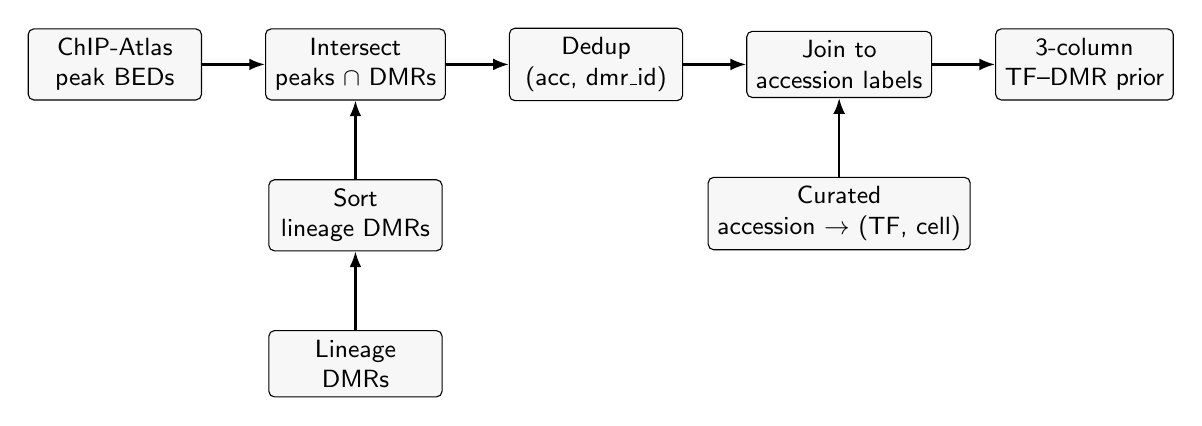
\begin{tikzpicture}[
      node distance=8mm and 8mm,
      box/.style={
        draw, rounded corners=2pt, minimum height=8mm,
        minimum width=22mm, align=center, font=\small\sffamily,
        fill=black!3
      },
      arrow/.style={-{Latex[length=2mm]}, thick}
    ]
    \node[box] (peaks) {ChIP-Atlas\\peak BEDs};
    \node[box, right=of peaks] (intersect) {Intersect\\peaks $\cap$ DMRs};
    \node[box, right=of intersect] (dedup) {Dedup\\(acc, dmr\_id)};
    \node[box, right=of dedup] (join) {Join to\\accession labels};
    \node[box, right=of join] (out) {3-column\\TF--DMR prior};
    \node[box, below=10mm of intersect] (sort) {Sort\\lineage DMRs};
    \node[box, below=10mm of sort] (dmrs) {Lineage\\DMRs};
    \node[box, below=10mm of join] (labels)
        {Curated\\accession $\to$ (TF, cell)};
    \draw[arrow] (peaks) -- (intersect);
    \draw[arrow] (intersect) -- (dedup);
    \draw[arrow] (dedup) -- (join);
    \draw[arrow] (join) -- (out);
    \draw[arrow] (dmrs) -- (sort);
    \draw[arrow] (sort) -- (intersect);
    \draw[arrow] (labels) -- (join);
  \end{tikzpicture}
  \caption{TF--DMR prior construction pipeline. ChIP-Atlas peak BEDs
  feed directly into the intersection and are shared across
  lineages; the lineage DMRs are sorted on their own path before
  the intersection. The lineage DMR BED and the curated accession
  label table are the lineage-specific and curation-specific inputs
  respectively.}
  \label{fig:pipeline_diagram}
\end{figure*}

\subsection{Curated TF set}
\label{sec:framework:tfset}

The curated TF set defines which ChIP-Atlas experiments enter the
TF--DMR prior. The curation procedure proceeds as follows. For each
(TF, cell type) combination that passes the curation criteria, the
three ChIP-Atlas experiments with the highest binding
enrichment are retained; this top-3 selection rule matches the
per-state TF assignment used
in the ChromHMM-based~\cite{ernst2017chromhmm} BICAN methylation
analysis~\cite{bican2026manuscript}. Taking the union of these
retained experiments across all (TF, cell type) combinations yields
the 172-record accession whitelist used as input to the TF--DMR
pipeline.
Because ChIP-Atlas aggregates experiments deposited in several
short-read archives, the curated accessions are not all
SRX-prefixed: they include SRX and ERX (and similar) accessions,
reflecting the archive in which each experiment was originally
deposited. The non-SRX accessions were part of the original
selection procedure rather than a separate addendum. In total the
curated set comprises 172~accessions, spanning SRX, ERX, and DRX
entries.

The exclusion criteria are applied upstream by the BICAN
ChromHMM-based selection that produces the 172-record accession
table; this work's pipeline inherits the resulting table and does not
re-filter it. The upstream curation removes categories of antigens
that appear in the ChIP-Atlas metadata but are not informative for
TF--DMR inference: antibody-tag entries (\texttt{Epitope},
\texttt{GFP}, \texttt{8-Hydroxydeoxyguanosine} and similar) that
reflect different experimental approaches where the TF target was
annotated in a different ChIP-Atlas metadata column, and
histone-modification antigens (\texttt{H3K27ac}, \texttt{H3K4me3},
\texttt{H3K9me3} and similar), which describe chromatin state rather
than sequence-specific binding. Inspection of the curated 172-record
table confirms that no histone-modification, antibody-tag, or
chemical-modification antigen remains in it; these exclusions are
inherited from the upstream curation rather than applied here.

The retained antigens are not exclusively sequence-specific
transcription factors. Most are sequence-specific TFs (for example
REST, SOX10, SOX2, ASCL1, NEUROD1, FOS, FOSL2, JUNB, the MEF2
family, and nuclear receptors such as NR3C1). The remainder are non-sequence-specific chromatin-associated
proteins that the top-3 binding-enrichment procedure
retained because they carry strong, localized ChIP-seq evidence: the
cohesin
subunits RAD21 and SMC1A, which form a structural, architectural
complex rather than a transcriptional cofactor; the Mediator
subunits MED1 and MED12, which form a transcriptional coactivator
complex; ATP-dependent SWI/SNF--BAF remodeler subunits (SMARCA4,
SMARCB1, SS18, BRD9); chromatin readers (BRD4, CBX2); chromatin- and
DNA-modifying enzymes (EP300, DNMT3A, SETD1A); and
transcription-elongation and RNA-associated factors (NELFE, SETX,
FUS, EWSR1). These are retained deliberately, as proteins whose
localized binding is informative about regulatory-element activity
at DMRs, but they are not sequence-specific regulators and are
described as such rather than as ``cofactors.'' One retained entry,
\texttt{BCL10}, appears in the curated set with three SRX accessions
in IMR90 cells (\texttt{SRX329082}, \texttt{SRX329084},
\texttt{SRX329085}). BCL10 is canonically a cytoplasmic signaling
adaptor of the CARMA1--BCL10--MALT1 complex with no established
sequence-specific or chromatin-associated role, so a ChIP-Atlas
``BCL10'' antigen assignment in a non-neural fibroblast line is
plausibly either a metadata-labeling issue or an atypical experiment;
the source publications behind these SRX records have not been
verified against the ChIP-Atlas experiment-list metadata here.
% TODO(jon): verify BCL10 source publication(s) against ChIP-Atlas
% experimentList.tab.gz and decide whether to drop these three SRX
% accessions from the curated set. The
curation is canonical across all five lineage outputs: the same
accession-to-(TF, cell) mapping is applied to every lineage, and the
final TF--DMR files exhibit zero label conflicts across the five
outputs.

\subsection{BrainSpan expression filter}
\label{sec:framework:brainspan}

ChIP-Atlas aggregates experiments across all available cell types and
tissues, so a TF can pass the curation step on the strength of
peaks in a non-brain context. The BrainSpan filter restricts the
prior to TFs that are expressed in developing human brain. The
filter rule is:
\begin{enumerate}
  \item Compute, for each row of the BrainSpan expression matrix,
        the mean RPKM across all 524 BrainSpan samples.
  \item For each gene symbol with multiple transcript-level rows,
        take the maximum mean RPKM across rows. A TF counts as
        expressed if any of its transcript rows meets the threshold.
  \item Retain a TF if its per-symbol mean RPKM exceeds the
        threshold.
\end{enumerate}

The threshold used is mean RPKM~$> 1.0$. Its rationale is the
borderline-regulator anchor point: REST, a transcriptional repressor
with well-characterized roles in neural lineage specification, has a
BrainSpan mean RPKM of~$1.29$, and the chosen threshold of $1.0$
lies below that value so REST is retained; a threshold above $1.29$
would have dropped REST despite its biological relevance, while
$1.0$ still excludes TFs that are not appreciably expressed across
the BrainSpan samples. The filter outcome is reported here on the
78-symbol \emph{gene-substrate analog reference}, an earlier and
looser TF set built from the same upstream BICAN selection but prior
to the antigen exclusions that produced the 172-record curated
accession set. The two sets are distinct: the looser 78-symbol
reference still contains the antibody-tag and chemical-modification
entries (\texttt{Epitope}, \texttt{GFP},
\texttt{8-Hydroxydeoxyguanosine}) that the upstream curation later
removed, whereas the final 172-record curated accession set used in
the DREM analysis already excludes them. Of the 78~unique TF symbols
in this analog reference, 58~pass the filter, 17~fall below the
threshold, and 3~are absent from the BrainSpan gene table entirely:
the antibody-tag antigens \texttt{Epitope} and \texttt{GFP}, which
have no gene-symbol counterpart in BrainSpan, and \texttt{KMT2D}, a
gene symbol not represented in the BrainSpan rows metadata. The analysis in this
report
uses a single prior variant: the annotated
\texttt{TF|cell|accession} prior, which is the file supplied to DREM
as its TF-interaction input. The BrainSpan filter operates on this
prior by extracting the TF symbol as the substring preceding the
first \texttt{|} in the first column. The regeneration script also
emits two further products that were \emph{not} used in the DREM
analysis: a TF-collapsed prior keyed by TF symbol only, and a
protein-coding-restricted variant of the annotated prior. The
protein-coding-restricted variant is kept only as a robustness
check; applying the same filter to it yields the same retained set,
because the protein-coding restriction is a strict subset of the
BrainSpan filter on the TF column.

\section{Implementation}
\label{sec:impl}

The pipeline is implemented as bash plus Python, with all genomic
operations delegated to \texttt{bedtools}~\cite{quinlan2010bedtools}
and the BrainSpan filter implemented in
\texttt{pandas}~\cite{mckinney2010pandas}. The full pipeline runs on
UCLA's Hoffman2 cluster; per-lineage runtime is dominated by the
\texttt{bedtools intersect} step over the ChIP-Atlas peak set, which
parallelizes naturally over accessions. The scripts that implement
each step are publicly available
(Section~\ref{sec:code})~\cite{paino2026repo}; rather than reproduce
the shell plumbing, this section gives pseudocode for the two steps
where the algorithm itself is the point.

Algorithm~\ref{alg:dmr_aggr} gives the per-cluster CpG aggregation
over DMRs that produces one column of the $\beta$-matrix described in
Section~\ref{sec:framework:matrix}. For each developmental-stage
cluster, CpGs are extracted from the allc file and mapped over the
sorted merged lineage DMR BED, the methylated and total reads are
summed and overlapping CpGs counted per DMR, and the per-DMR sums
are converted into a coverage-weighted $\beta$ value.

\begin{algorithm}[t]
\caption{Per-cluster coverage-weighted $\beta$ over the merged
  lineage DMR BED (implemented in \texttt{apm\_<lineage>\_DMR.sh}).}
\label{alg:dmr_aggr}
\begin{algorithmic}[1]
\Require sorted merged lineage DMR BED $D$; sorted per-cluster CpG
  records, each overlapping CpG $i$ carrying methylated reads $m_i$
  and total reads $C_i$
\Ensure per-DMR $\beta$ for this cluster
\For{each DMR $d \in D$}
  \State $M_d \gets \sum \{\, m_i : \text{CpG } i \text{ overlaps } d \,\}$
  \State $T_d \gets \sum \{\, C_i : \text{CpG } i \text{ overlaps } d \,\}$
  \State $n_d \gets |\{\, i : \text{CpG } i \text{ overlaps } d \,\}|$
  \If{$T_d = 0$ \textbf{ or } $n_d = 0$}
    \State $\beta_d \gets \textsc{na}$
  \Else
    \State $\beta_d \gets M_d / T_d$
  \EndIf
\EndFor
\State \Return $\{(d, \beta_d) : d \in D\}$
\end{algorithmic}
\end{algorithm}

Algorithm~\ref{alg:intersect} gives the core peak-DMR intersection.
For each whitelisted accession, the peak BED is intersected with the
sorted DMR set, the (accession, DMR identifier) pair is emitted for
every overlap, and the cumulative output is deduplicated.

\begin{algorithm}[t]
\caption{Peak-DMR intersection (implemented in
  \texttt{regenerate\_tf\_dmr.sh}).}
\label{alg:intersect}
\begin{algorithmic}[1]
\Require whitelisted accessions $A$; per-accession peak BED $B_a$;
  sorted merged lineage DMR BED $D$
\Ensure deduplicated set of (accession, DMR) pairs
\State $S \gets \emptyset$
\For{each accession $a \in A$}
  \For{each peak $p \in B_a$ overlapping some DMR $d \in D$}
    \State $S \gets S \cup \{(a,\ \mathrm{id}(d))\}$
  \EndFor
\EndFor
\State \Return $S$
\end{algorithmic}
\end{algorithm}

The BrainSpan filter follows the enumerated rule of
Section~\ref{sec:framework:brainspan}: the expression matrix is
averaged row-wise across all 524 samples, the row means are joined to
the gene-symbol metadata, the maximum mean across transcript-level
rows is taken per gene symbol, and TFs are retained where the
per-symbol mean exceeds the threshold.

Listing~\ref{lst:beta_matrix} shows an excerpt of the OPC--ODC
$\beta$-matrix produced by the pipeline of
Section~\ref{sec:framework:matrix}. Rows are DMRs and columns are
developmental-stage clusters in lineage order; each cell is the
coverage-weighted $\beta$ for that DMR in that cluster. The matrix
is the dynamic-input layer that DREM observes for the lineage.

\begin{lstlisting}[
  float=*tp,
  style=tsvstyle,
  caption={Excerpt of the OPC--ODC DMR $\beta$-matrix
    (\texttt{OPC\_ODC\_dmr\_beta.matrix.tsv}). Rows are DMRs;
    columns are developmental-stage clusters in lineage order;
    cells are coverage-weighted methylation $\beta$-values.
    Empty cells (omitted in this excerpt) indicate that no
    CpG within the DMR had coverage in the corresponding cluster.},
  label={lst:beta_matrix}
]
                              2T_GPC  GPC     OPC     tOPC    tODC    ODC     adult_ODC
dmr_chr1_117587864_117588098  1       0.9545  0.0111  0.0172  0       0.0168  0.2190
dmr_chr10_96560195_96560440   1       0.8247  0.1667  0.0968  0       0.0563  0.1474
dmr_chr11_27669278_27669395   1       0.8333  0.1698  0.0769  0.1667  0       0.0588
\end{lstlisting}

Listing~\ref{lst:format} shows the resulting 3-column TF--DMR prior
file format. The first column carries the annotated
\texttt{TF|cell|accession} key; the second column is the DMR
identifier that the merged lineage DMR BED assigns to the
overlapping region; the third column is the binary input value that
DREM's logistic regression at the split nodes consumes. The
accession in the excerpt below (\texttt{DRX190656}) is itself a
non-SRX accession, illustrating that the curated set spans multiple
short-read archives.

\begin{lstlisting}[
  style=tsvstyle,
  caption={Excerpt of the regenerated MGE\_PVALB TF--DMR prior file.
    Each row records that experiment \texttt{DRX190656} for TCF21 in
    HCF cells has a ChIP-Atlas peak overlapping the named DMR
    in the MGE\_PVALB lineage.},
  label={lst:format}
]
TF                          Gene                                Input
TCF21|HCF|DRX190656         dmr_chr10_102208297_102209008       1
TCF21|HCF|DRX190656         dmr_chr10_103771954_103772499       1
TCF21|HCF|DRX190656         dmr_chr10_11242443_11242850         1
\end{lstlisting}

\section{Results}
\label{sec:results}

The BrainSpan filter outcome on the analog gene-substrate reference
(78 unique TF symbols; 58 retained, 17 below threshold, 3 absent
from BrainSpan) is reported in
Section~\ref{sec:framework:brainspan}; this section focuses on the
downstream effect of the regenerated TF--DMR prior on the fitted
DREM models.

\begin{figure*}[t]
  \centering
  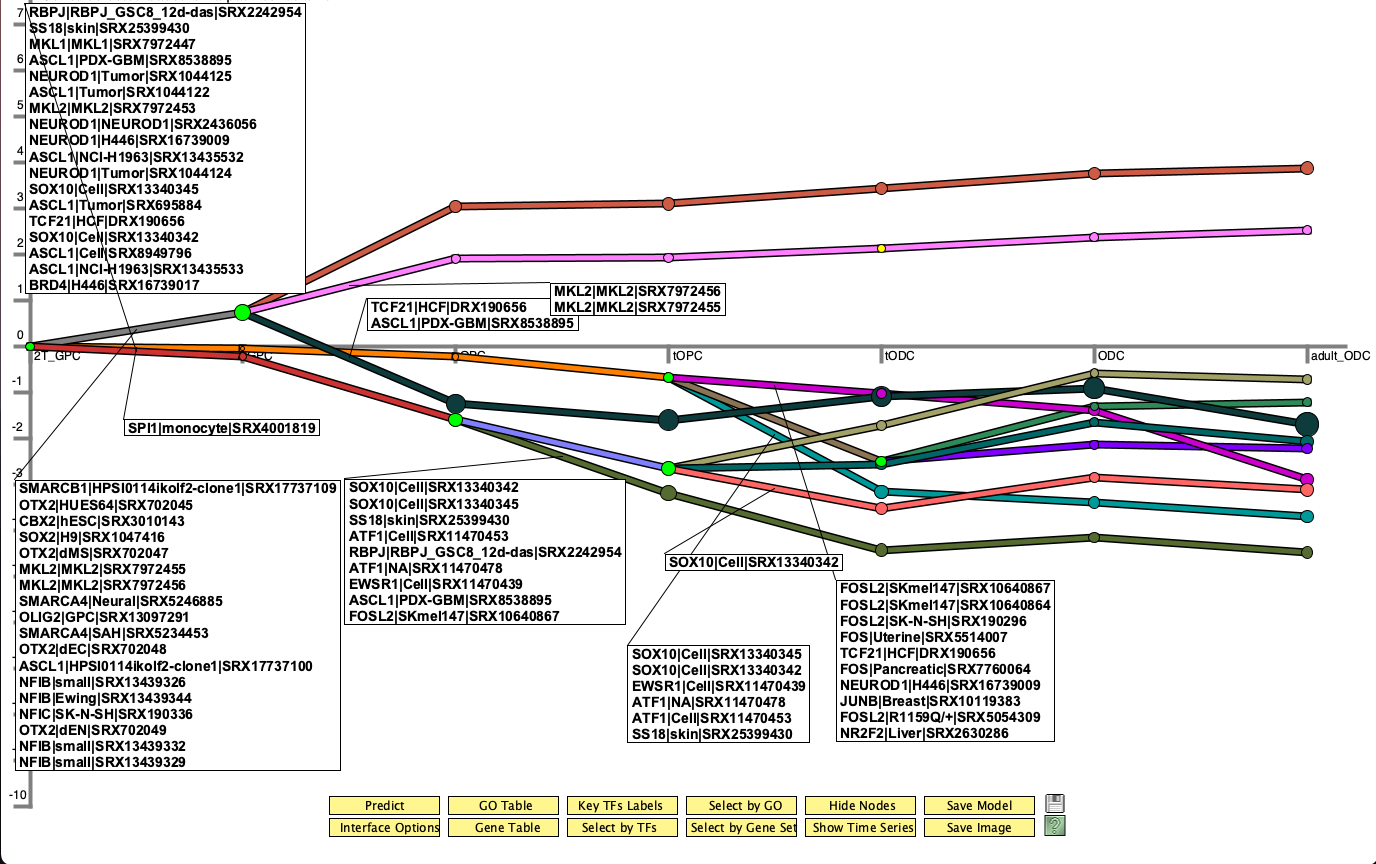
\includegraphics[width=\linewidth]{opc-odc-figure/drem-opc-odc.png}
  \caption{DREM model fit for the OPC--ODC trajectory using the
  regenerated TF--DMR prior. Developmental stages advance
  left-to-right across the lineage (2T\_GPC, GPC, OPC, tOPC, tODC,
  ODC, adult\_ODC). Split nodes are annotated with the transcription
  factors whose targets are significantly enriched, by DREM's
  hypergeometric test, among the genes assigned to an outgoing path
  relative to the genes entering the split.}
  \label{fig:drem_opc_odc}
\end{figure*}

The DREM model fit for the OPC--ODC trajectory using the regenerated
TF--DMR prior is shown in Figure~\ref{fig:drem_opc_odc}. The model
spans seven developmental stages from second-trimester glial
progenitor cells (2T\_GPC) through progenitor and committed
populations (GPC, OPC, tOPC, tODC) to mature and adult
oligodendrocytes (ODC, adult\_ODC), and resolves a primary
bifurcation at the earliest stage transition that separates
regulatory elements demethylating across the lineage (upper paths)
from those gaining mCG (lower paths). Quantitatively, this model is
an IOHMM fit over 50{,}000 input DMRs, with 47 nodes in total: 6
split nodes (two two-way and four three-way) and 11 terminal paths.
At each split, candidate TFs are scored by DREM's hypergeometric
enrichment test and are retained as path annotations when the
enrichment passes the split significance threshold of $p \leq
10^{-3}$ (DREM's
\texttt{Key\_Input\_X\_p-val\_10\textasciicircum{}-X} parameter set
to $3.0$, with significance basis
\texttt{Path Significance Conditional on Split});
$61$ TF annotations are assigned across the six splits.

At the upper, demethylating split, the DREM model annotates the
bifurcation with SOX10, NEUROD1, ASCL1, and TCF21 as significant
regulators, drawing on the TF--DMR prior. A single ChIP-Atlas
experiment is sufficient for SOX10 to be called at this split; here
it is supported by multiple experiments, which is corroborative
rather than required. SOX10 is also annotated independently at the
OPC-to-tOPC and tOPC-to-tODC splits, indicating that the regenerated
prior captures SOX10 binding enrichment at progressively
demethylating regulatory elements across both OPC commitment and ODC
maturation rather than only at the lineage-defining bifurcation. This
identifies SOX10 as a lineage-specific driver of demethylation along
the OPC--ODC trajectory, consistent with the role reported in the
BICAN methylation manuscript~\cite{bican2026manuscript} and with
SOX10's established requirement for terminal oligodendrocyte
differentiation and
myelination~\cite{stolt2002sox10,emery2015oligodendrocyte}, and adds
the observation that the signal is sustained across multiple
intra-lineage transitions.

At the lower, methylation-gaining split, the model annotates the
bifurcation with SMARCB1, SMARCA4, SOX2, OTX2, OLIG2, and NFIB. The
SMARCA4 and SMARCB1 enrichments at regions gaining mCG in
mid-gestational development are consistent with SWI/SNF
chromatin-remodeler binding at sites where polycomb repression is
progressively replaced by de novo
methylation~\cite{bican2026manuscript,stanton2017smarca4}. The
co-enrichment of SOX2
and ASCL1 at the same path is consistent with early patterning TF
binding sites gaining mCG in
mid-gestation~\cite{bican2026manuscript}. OLIG2 and NFIB at this
path are consistent with pro-glial factor binding sites accumulating
methylation during cell-fate commitment~\cite{bican2026manuscript},
here visible from within the glial trajectory itself: regulatory
elements bound by OLIG2 in glial progenitors silence as cells commit
further along the OPC--ODC arc.

\begin{figure*}[t]
  \centering
  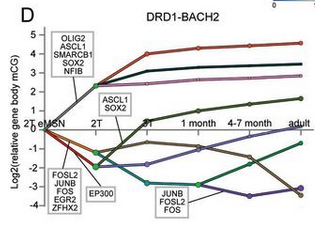
\includegraphics[width=0.45\linewidth]{bach2.png}
  \caption{DREM model fit for the DRD1-BACH2 trajectory using the regenerated TF--DMR prior.
    Developmental stages advance left-to-right across the lineage.
    Split nodes are annotated with the transcription factors whose
    targets are significantly enriched, by DREM's hypergeometric
    test, among the genes assigned to an outgoing path relative to
    the genes entering the split.}
  \label{fig:drem_bach2}
\end{figure*}

\begin{figure*}[t]
  \centering
  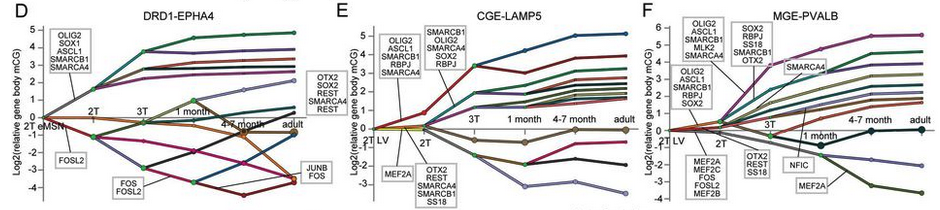
\includegraphics[width=\linewidth]{epha4-lamp-pvalb.png}
  \caption{DREM model fits for the DRD1-EPHA4 , eCGE-LAMP5, and MGE-PVALB trajectories using the
    regenerated TF--DMR priors. Each panel shows one lineage with
    developmental stages advancing left-to-right. Split nodes are
    annotated with the transcription factors whose targets are
    significantly enriched, by DREM's hypergeometric test, among the
    genes assigned to an outgoing path relative to the genes
    entering the split.}
  \label{fig:drem_msn_cge_mge}
\end{figure*}

The remaining four lineages were fit with the same pipeline.
Figure~\ref{fig:drem_bach2} shows the DRD1-BACH2 striosomal MSN
trajectory; Figure~\ref{fig:drem_msn_cge_mge} shows the DRD1-EPHA4
matrix MSN, eCGE-LAMP5, and MGE-PVALB trajectories.

In DRD1-BACH2 (striosomal MSN; Figure~\ref{fig:drem_bach2}), the
splits carry AP-1 family annotations (FOSL2, FOS, JUNB) at regions
demethylated during mid-gestation, consistent with the BICAN finding
that striosomal MSNs show earlier and stronger activity-dependent
AP-1 enrichment than matrix MSNs~\cite{bican2026manuscript}.

In DRD1-EPHA4 (matrix MSN; Figure~\ref{fig:drem_msn_cge_mge}), AP-1
enrichment in mid-gestation is comparatively absent relative to
DRD1-BACH2; instead the mid-gestational regions of methylation
change are enriched for MEIS, PBX, and PKNOX family motifs, again
per the BICAN matrix-MSN
characterization~\cite{bican2026manuscript}.

In eCGE-LAMP5 (Figure~\ref{fig:drem_msn_cge_mge}), the DREM fit
annotates its splits with CGE inhibitory-neuron regulators; where
the figure resolves specific factors, these include DLX-, ARX-, and
SOX-family transcription factors associated with CGE-derived
interneuron specification.

In MGE-PVALB (Figure~\ref{fig:drem_msn_cge_mge}), the splits along
the trajectory carry MEF2C together with MGE-defining transcription
factors (LHX6, MAF), consistent with the abstract's identification
of MEF2C as a lineage-specific driver of methylation change in the
MGE-derived inhibitory neuron arc~\cite{bican2026manuscript}.

Taken together, the DREM fits across the five lineages produced by
the TF--DMR prior pipeline yield biologically coherent split
annotations: a demethylating arc dominated by SOX10 and other
glial-lineage regulators in OPC--ODC; a methylation-gaining arc
carrying SWI/SNF and early patterning factors in OPC--ODC; AP-1
family enrichment differentiating striosomal from matrix MSN
trajectories; and MEF2C and MGE-defining TFs at the MGE-PVALB
splits. These are standalone findings of the pipeline rather than a
reproduction of any prior model. The OPC--ODC fit additionally
resolves SOX10 enrichment across three successive intra-lineage
splits. One caveat applies to
all of these calls: the top-3 selection rule itself bounds TF
coverage, so the annotations reflect only TFs with enough average
binding enrichment in ChIP-Atlas to clear that cutoff; relaxing
the top-3 restriction would admit additional candidate TFs at every
split.

\section{Discussion and Limitations}
\label{sec:discussion}

The TF--DMR prior framework is constrained by ChIP-Atlas coverage.
A TF can only enter the prior if it has enough public ChIP-seq
accessions to clear the top-3 selection criterion, regardless of
its biological importance. TFs with no ChIP-seq evidence in
ChIP-Atlas are absent from the prior even when there is independent
evidence of their role in a lineage; this is a limitation inherited
from the underlying TF binding evidence base, not from the prior
construction itself. The top-3 rule is itself a restriction, not
only a coverage floor: relaxing it (retaining more than three
experiments per (TF, cell type) combination, or lowering the
binding-enrichment bar) would admit additional TFs into every
lineage prior, at the cost of including experiments with lower
binding enrichment.

The BrainSpan expression filter assumes that brain-wide bulk RPKM is
a reasonable proxy for whether a TF is operative in any specific
lineage. This is conservative in the right direction (a TF that is
unexpressed across all 524 BrainSpan samples is unlikely to be
operative in any lineage), but it does not distinguish between TFs
that are broadly expressed and TFs that are sharply lineage-specific.
A lineage-specific expression filter built from per-cell-type
expression data would refine the prior further and is a natural next
step.

The prior is binary at the TF level after collapse. The 3-column
DREM input format admits continuous values in the third column, and
DREM 2.0~\cite{schulz2012drem2} can in principle consume the
ChIP-Atlas peak score as a continuous binding intensity. The current
TF--DMR prior discards that information, treating an overlap as a
binary indicator. Reintroducing the peak-strength signal is a
mechanical change to the construction script but would require
calibrating the input scale against the existing IOHMM logistic
regression behavior.

DMR calling is performed upstream by the BICAN methylation pipeline
and is not part of the framework presented here. The TF--DMR prior
inherits whatever DMR-calling assumptions were used for the merged
lineage DMR BEDs: developmental-stage binning, the pairwise
between-stage comparison, coverage filters, methylation-difference
thresholds, and the union-merging strategy.
Changes to those upstream choices would propagate into a different
DMR set and therefore a different prior, even with no change to the
construction script.

\section{Future Work}
\label{sec:future}

The same prior-construction infrastructure used here for methylation
extends to scRNA-seq lineage trajectories. In that setting, the
dynamic substrate is gene expression aggregated to the lineage
trajectory clusters (the same developmental-stage / trajectory
clustering used to order the methylation columns, not a separate
pseudotime binning), and the prior reverts to a TF-to-gene
table. The construction differs from the standard DREM workflow
primarily in the accession curation and, where applicable, the
BrainSpan filter. The accession curation transfers unchanged to any
system; the BrainSpan filter transfers only when the new system is
also a developing-brain context. For a non-brain atlas such as
IGVF, BrainSpan is not an appropriate relevance filter and would be
replaced by an expression reference matched to that system. That arm
of the work is in progress with collaborator-provided trajectory
data and will be reported separately in an in-progress writeup.

\section{Summary}
\label{sec:summary}

DREM's IOHMM is agnostic about the substrate of its dynamic input as
long as the prior establishes a correspondence between transcription
factors and the entities indexed in the dynamic matrix. The TF--DMR
prior framework realizes that observation for the BICAN methylation
analysis: it replaces the standard TF-to-gene prior with a
TF-to-DMR prior, restricts the TF coverage with a curated accession
whitelist (172 records, spanning SRX, ERX, and DRX entries) and a
BrainSpan RPKM filter, and produces all five lineage-specific priors
from a single parameterized regeneration pipeline. The framework also
provides a working test of whether DREM remains functional with
methylation, rather than expression, as the dynamic substrate. The
regenerated priors retain the biologically anchored borderline
regulators that motivated the threshold choice and yield DREM fits
across all five lineages with biologically coherent split
annotations, including SOX10 enrichment resolved across multiple
intra-lineage splits in OPC--ODC and AP-1 enrichment distinguishing
striosomal from matrix MSN trajectories.

\section{Code Availability}
\label{sec:code}

The scripts implementing the pipeline described in this report are
publicly available at
\url{https://github.com/ernstlab/drem-bican-tfdmr}~\cite{paino2026repo}.
The repository contains the per-lineage DMR $\beta$-matrix
construction scripts (\texttt{apm\_*\_DMR.sh},
\texttt{combine\_filtered\_methylation\_*.sh}), the TF--DMR prior
builder and its driver (\texttt{regenerate\_tf\_dmr.sh},
\texttt{run\_all\_lineages.sh}), and the BrainSpan RPKM TF filter
(\texttt{brainspan\_filter\_tf\_prior.py}), with a README documenting
each script and the pipeline order, together with a \texttt{paper/}
directory holding the \LaTeX{} source and compiled PDF of this
report. It contains code and writeup source only: the BICAN-derived
inputs and outputs are not redistributed there, as the underlying
atlas is unpublished.

\begin{acks}
The author thanks Jason Ernst for advising this work; Chongyuan Luo,
Runjia Li, and
Terence Li for the BICAN methylation data,
trajectory definitions, and the ChromHMM-derived ChIP-Atlas curation
on which the TF--DMR priors are built; and the broader team that
generated the developing human brain
atlas~\cite{bican2026manuscript}.
\end{acks}

\bibliographystyle{ACM-Reference-Format}
\bibliography{references}

\end{document}
